\section{Hardware}
In diesem Kapitel wird die Hardware der Steuerung im Detail erläutert.

% \begin{itemize}
%     \item Beschreibung, Zweck der TECs
%     \item Beschreibung der TECs und wo diese platziert sind mit Illustrationen
% \end{itemize}

\subsection{Komponenten}
\begin{figure}[H]
    \centering
    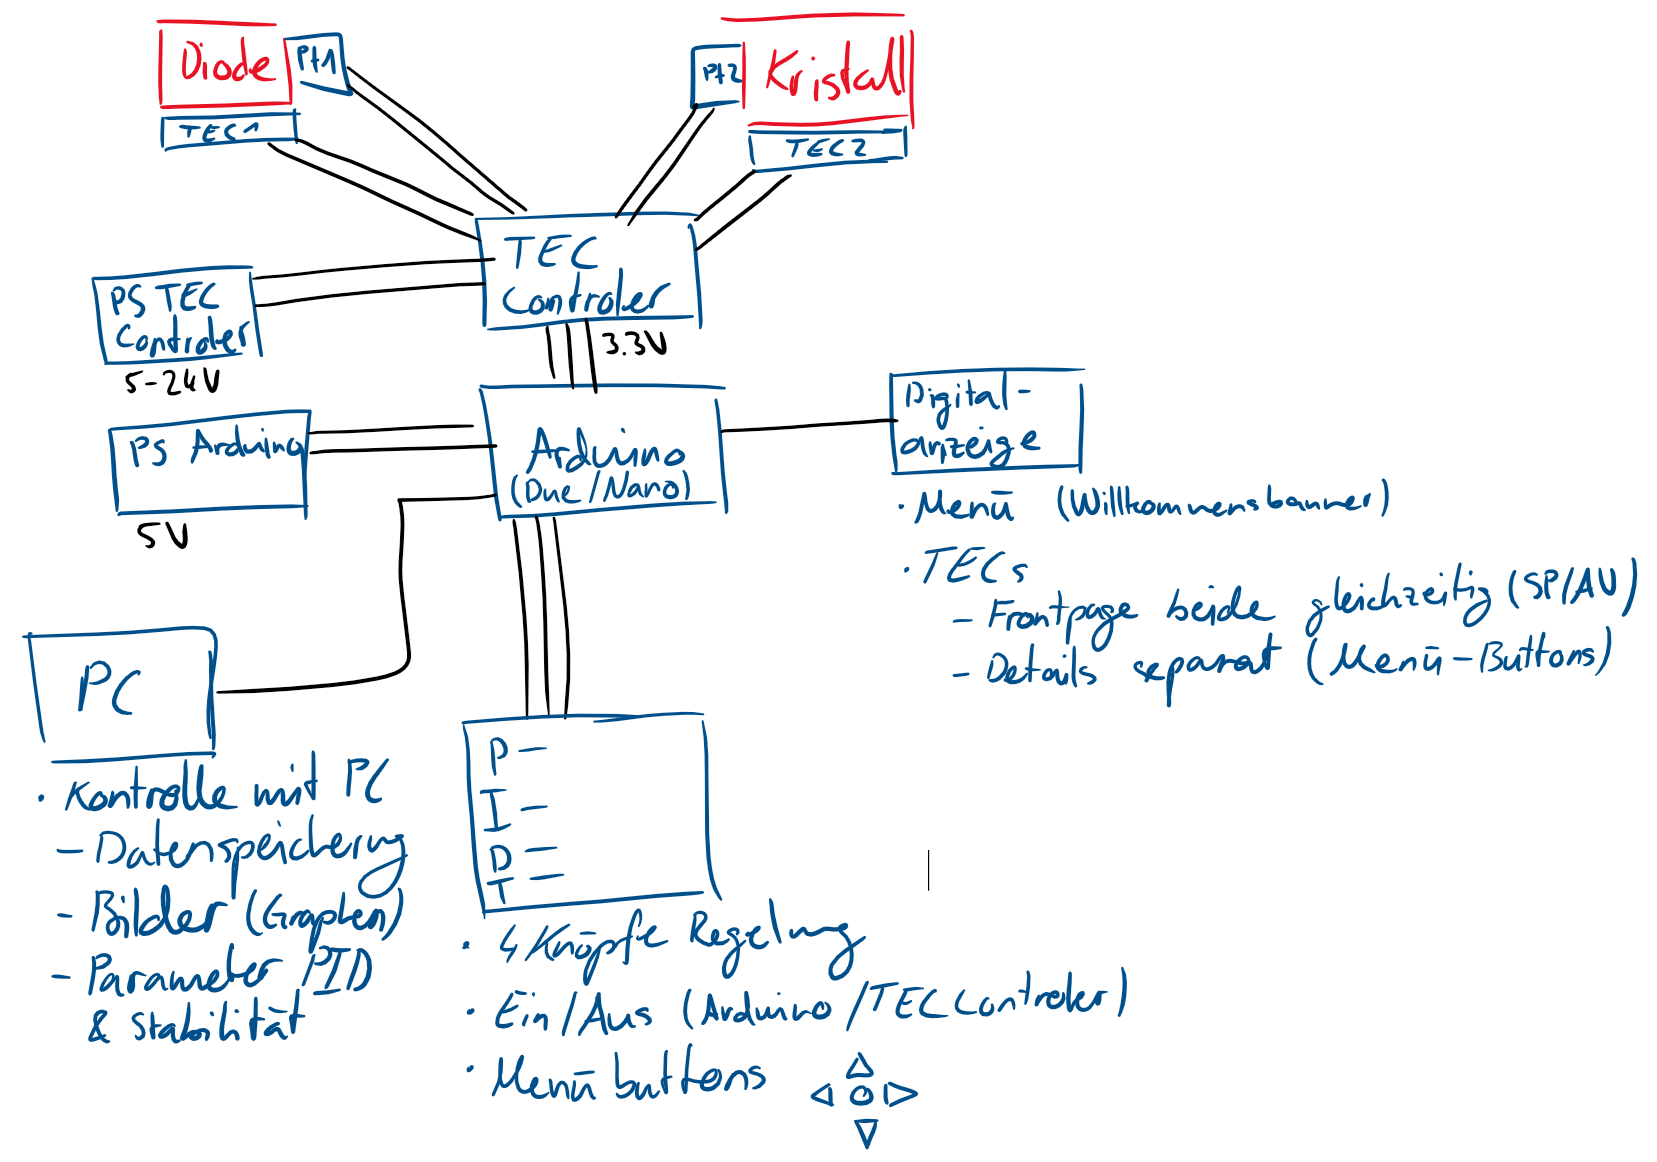
\includegraphics[scale=0.5]{98_images/scheme_wiring.PNG}
    \caption{Verkabelung der elektrischen Komponenten.}
    \label{fig:scheme_wiring}
\end{figure}

\subsection{Energieversorgung}  % $-$ PS}
Die benötigte Leistung des Netzteils für das gesamte System beläuft sich auf etwa 80W.
Dies wurde einerseits errechnet (s. Anhang \ref{formula:_calculation_sp_power}), andererseits mit einem Netzteil an dem alle Komponenten angeschlossen waren verifiziert.


\begin{figure}[H]
    \centering
    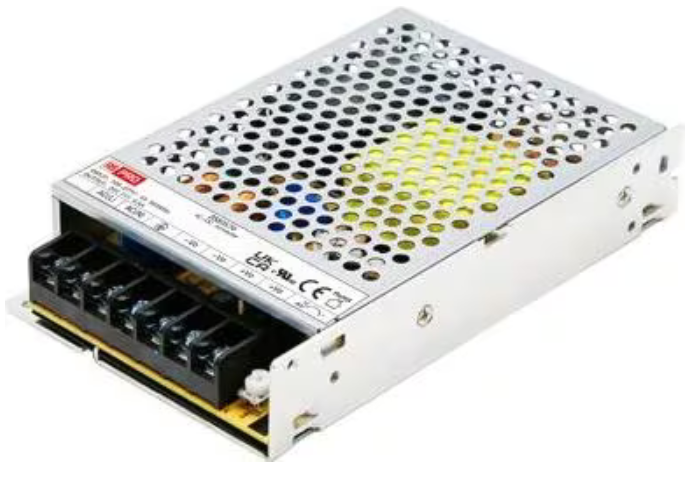
\includegraphics[scale=0.7]{98_images/controller_ps.PNG}
    \caption{Ausgewähltes Netzteil der Marke RS auf Grund der Berechnung 4.1. Es Liefert 24V und 6.5A. Dies entspricht der benötigten Energieversorgung und kann spätere Erweiterungen oder Änderungen aufnehmen.}
    \label{fig:enter-label}
\end{figure}

\subsection{Sensorik}
Die Positionen der Temperaturmessung des Alexandritkristalls und der Diode sind in Abbildung \ref{} dargestellt. An diesen Positionen stören sie den Laser im Betrieb nicht und können trotzdem die Temperatur möglichst nahe an der Quelle messen.

\begin{figure}
    \centering
    % \includegraphics{}
    \caption{Caption}
    \label{fig:enter-label}
\end{figure}

\subsection{Verkabelung}  % Architektur der Verkabelung
Die externe Verkabelung des Gehäuses bzw. dessen Komponenten, erfolgt mit einem XYZ-Kabel. Somit können alle Komponente die zum Laser gehen kompakt in einem Kabel geführt werden.\\
Intern werden die Komponente mit einem XYZ-Kabel verdrahtet und werden über einen Kabelbaum geführt.\textbf{NICHT NÖTIG!!!!!!!!!!}\\

\textbf{Auswahl der Digitalanzeige}
Für die Digitalanzeige waren vor allem drei Aspekte ausschlaggebend, um die gewünschte Funktion zu gewährleisten. Die Eingabe der Werte, die Anzeige der Werte und Verständlichkeit der angezeigten Werte. All die Kriterien sollten erfüllt werden, um die Steuerung des Lasers gewährleisten.

\begin{table}[H]
    \centering
    \begin{tabular}{l|l}
        \textbf{16x2 mit Taster}&       \textbf{800x400 Touchanzeige}\\
        $-$ Taster Analogeingänge&      $+$ ntegriert\\
        $-$ Kleine Anzeige&             $+$ Grössere Anzeige\\
        $-$ Kryptische Anzeige&         $+$ Verständliche Anzeige\\
        $-$ Tieferes Menü&              $+$ Weniger tiefes Menü\\
        $+$ Einfache Programmierung&    $-$ Anspruchsvolle Programmierung\\
    \end{tabular}
    \caption{Pro - Kontra Liste für die Auswahl der Digitalanzeige}
    \label{tab:choice_display}
\end{table}

Die Entscheidung fiel auf die Touchanzeige. Zusätzlich lassen sich alle Komponente wie Knöpfe direkt in die Anzeige programmieren. Es müssen keine komplexen Abläufe programmiert werden, die die Betätigung der physischen Knöpfe erkennt und das Programm lenkt. Zusätzlich müssen keine Ein-/Ausgänge zusätzlich auf der SPS einprogrammiert werden. Mit der Anzeige können ganze Designs erstellt werden, was das Arbeiten mit der Steuerung ergonomischer macht.  

\subsection{Konstruktion des Gehäuses}
Das Gehäuse war bereits vorhanden. Die im Kapitel XYZ aufgelisteten Komponenten wurden auf zusätzlichen Blechen montiert. Durch die Form des Gehäuses entstand so mehr Fläche für die Komponenten und vereinfachte dadurch die Montage. Zusätzlich mussten noch die Zugänge für die Verkabelung der Stromversorgung, deren Schalter und das Kabel für die Ansteuerung der Komponenten im Laser-Aufbau angepasst werden.

\subsection{Testaufbau $-$ Mock-up}
In einem Mock-up konnten die Funktionen und das Verhalten der Steuerung geprüft werden. Darunter wurde getestet, ob die Temperaturen in der Steuerung im Rahmen bleiben. Gemessen werden die Temperaturen mit der internen Temperaturmessung des Prozessors des Raspberry PI. Die Temperatur im Gehäuse wurde dann von der Temperatur des Prozessors abgeleitet. Dafür wurde sie mit einem Temperaturmessgerät extern gemessen und die Messergebnisse mit denen des Prozessors verknüpft.
Die Positionen der Komponenten im Gehäuse wurde mit Hilfe von CAD-Software geprüft. Dafür wurden die oben genannten Bleche erstellt und die Komponente mit Verschraubungen platziert.

\lstdefinestyle{custompython}{
  belowcaptionskip=1\baselineskip,
  breaklines=true,
  frame=L,
  xleftmargin=\parindent,
  numbers=left,
  language=Python,
  showstringspaces=false,
  basicstyle=\footnotesize\ttfamily,
  keywordstyle=\bfseries\color{green!40!black},
  commentstyle=\itshape\color{purple!40!black},
  identifierstyle=\color{blue},
  stringstyle=\color{orange},
}

%\lstinputlisting[caption=Ein kurzes Codebeispiel in der Programmiersprache Python, style=custompython]{listings/python_example.py}
